\section{New Results 2023-06-12}

	\begin{figure}[H]
		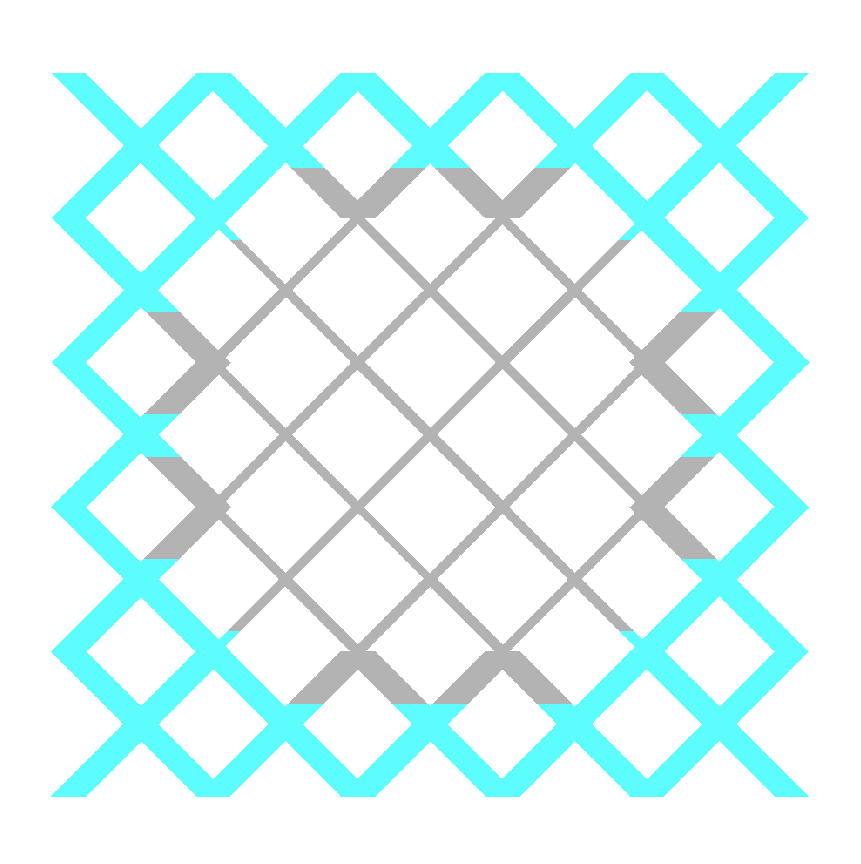
\includegraphics[height=8cm]{fig_result10by10_1}
		\caption{Initial setup, outer radius is 3 times larger than inner.}
		\label{fig_invasion-result1}
	\end{figure}
	
	\begin{figure}[H]
		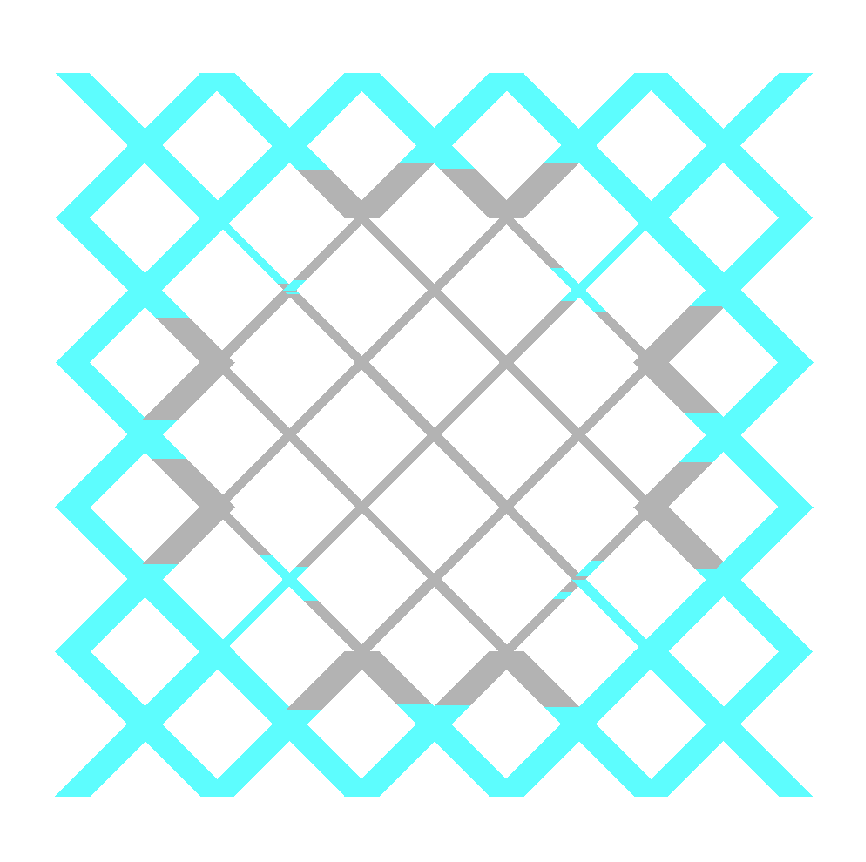
\includegraphics[height=8cm]{fig_result10by10_2}
		\caption{Showing invasion of wetting(blue) fluid into the region which contains thinner radius. The flow acclerates because, for a corner initially there are 3 meniscus, it multiplies into 3 when the meniscus reaches the node. The corner where the meniscus reaches the node late is pushed back because of the excessive pressures from the other corners.}
		\label{fig_invasion-result2}
	\end{figure}
	
	
	\begin{figure}[H]
		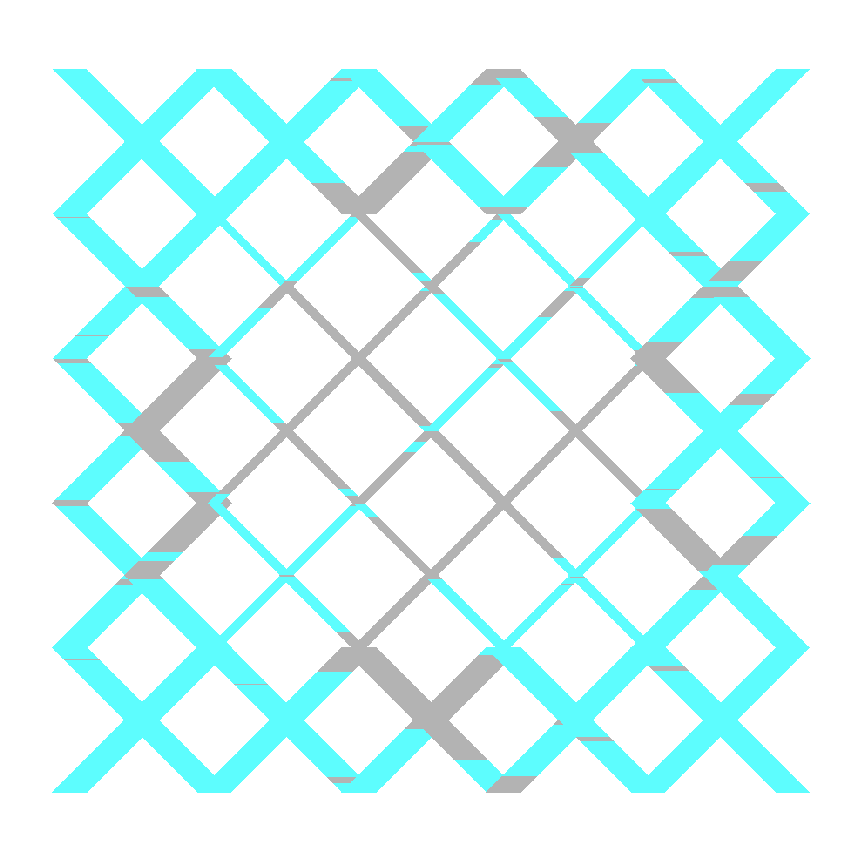
\includegraphics[height=8cm]{fig_result10by10_3}
		\caption{The invasion slows down and possibly ossicilates, it is due to the meniscus in the inner region being ineffective to suck more blue fluid as most tubes have two meniscus. In our algorithm, tubes with two meniscus have a zero net pressure.}
		\label{fig_invasion-result3}
	\end{figure}
	
	\begin{figure}[H]
		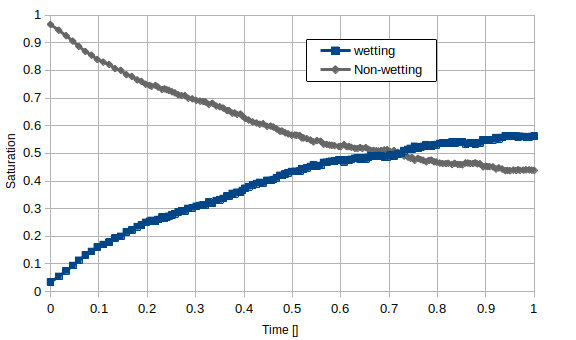
\includegraphics[width=16cm]{fig_plot-sat-vs-time}
		\caption{Plot of saturation of blue fluid in the region of thinner radius with respect to time, here the dimension of time is arbitary.}
		\label{fig_plot-sat-vs-time}
	\end{figure}
	
	\subsection{Discussion}
		There may be minor inaccuracies in the code, mostly in the part of distributing phases in the nodes. Even if there are minor mistakes. 
		\begin{enumerate}
			\item The total volume for each phase for the whole system remains the same with the accuracy of $10^-9$.
			\item The blue fluid has approximately logarithmic dependence with time, the invasion rapidly rises and slows down, until it becomes almost constant. The calculation was stopped after 150 steps, becasue there was very small progress after it. Note that the time step for each step is different.
			\item The blue fluid enters upto $0.56$ of the saturation.
			\item The saturation vs time appears similar to the ones in the reference [1], [2].
		\end{enumerate}

	\subsection{Initial conditon}
		\begin{enumerate}
			\item All calculations are done in double.
			\item For $K = 0.2$  the size of time-step. Or, if the velocity of all tubes were equal for all moment of time, then it would take $5$ steps for all initial fluid to flow out of a tube.
			\item To save time for now, it was done on a 10x10 tubes.
			\item Allowing 2 tubes on the outer, the saturation of blue was 0.77 while saturation of grey was 0.22 for the whole system, if we make the size bigger like 30x30 then we can achieve a number closer to 0.50, 0.50 which we ilitially wanted. 
			\item Random numbers were added to the radius, the inner radius are approximately 3 times smaller than the outer radius. The random value changed a maximum of $0.01$.
			\item The node at the centre was chosen to have 0 pressure. Which is necessary for the linear equations to have a solution.
			\item blue,grey,blue,grey was combined to blue,grey,blue.
			\item viscosities of both fluids are equal
		\end{enumerate}
		
		
\section{Old Results, shown at the 65 mipt conference}

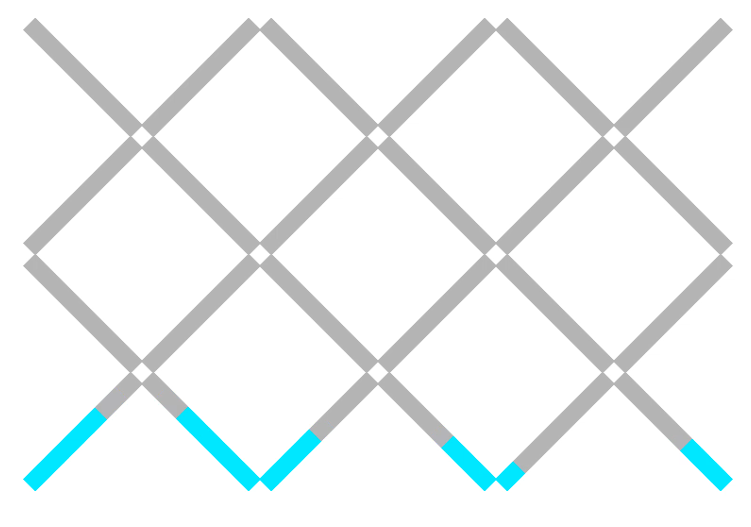
\includegraphics[height=6cm]{fig_initial-fill-distribution}


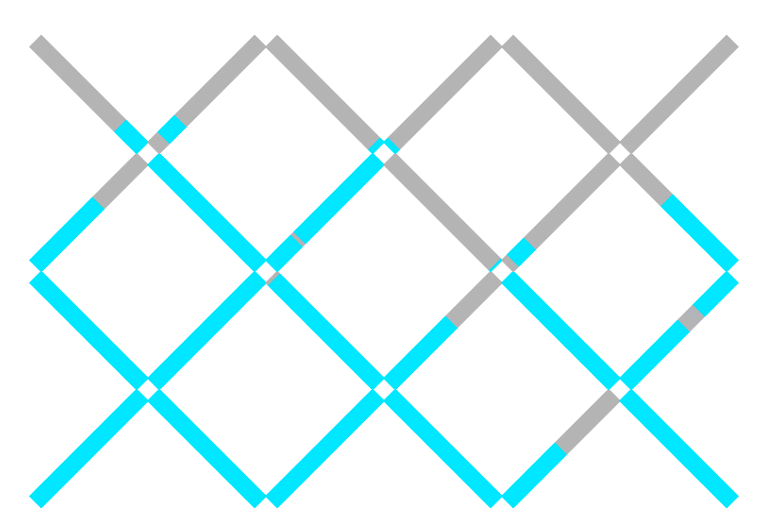
\includegraphics[height=6cm]{fig_final-fill-distribution}

Our model is initially set up such that the wetting fluid is low in saturation and is confined to the bottom of our network. A higher pressure is fixed for all nodes at the bottom layer, while a  low pressure is fixed for the top row. In all nodes, law of conservation of volume is applied, since mass is conserved and the phases are non-compressible. However for the bottom layer of nodes, the wetting fluid is injected as much required according to the sum of flow rates determined in the tubes connected to those nodes, while from the top layer of nodes a fluid is removed.

